\section{Background}
  To interface to the go-kart, actuators were required to be placed at the front
  of the kart, as well as interfacing to the power electronics in the rear. To
  allow high speed, computationally intensive signal processing, the control
  system is also required to be able to interface to a computer. This computer
  will be used to run computer vision code making use of image sensors.

\subsection{The Go-kart}
  The department has 5 electric go-karts that were purchased for the specific
  purpose of a assignment and project platform, one of these shown in Fig.
  \ref{go-kart}. Throughout the year several, mostly power electronics,
  assignments are based on the Junoir Sport JS80IIR go-kart. These go-karts are
  1.7 meters in length, can hold two passangers and came with a 80cc petrol
  motor. The petrol motor has since been replaced with a DC electric motor and
  batteries.

  \begin{figure}[h]
      \centering
      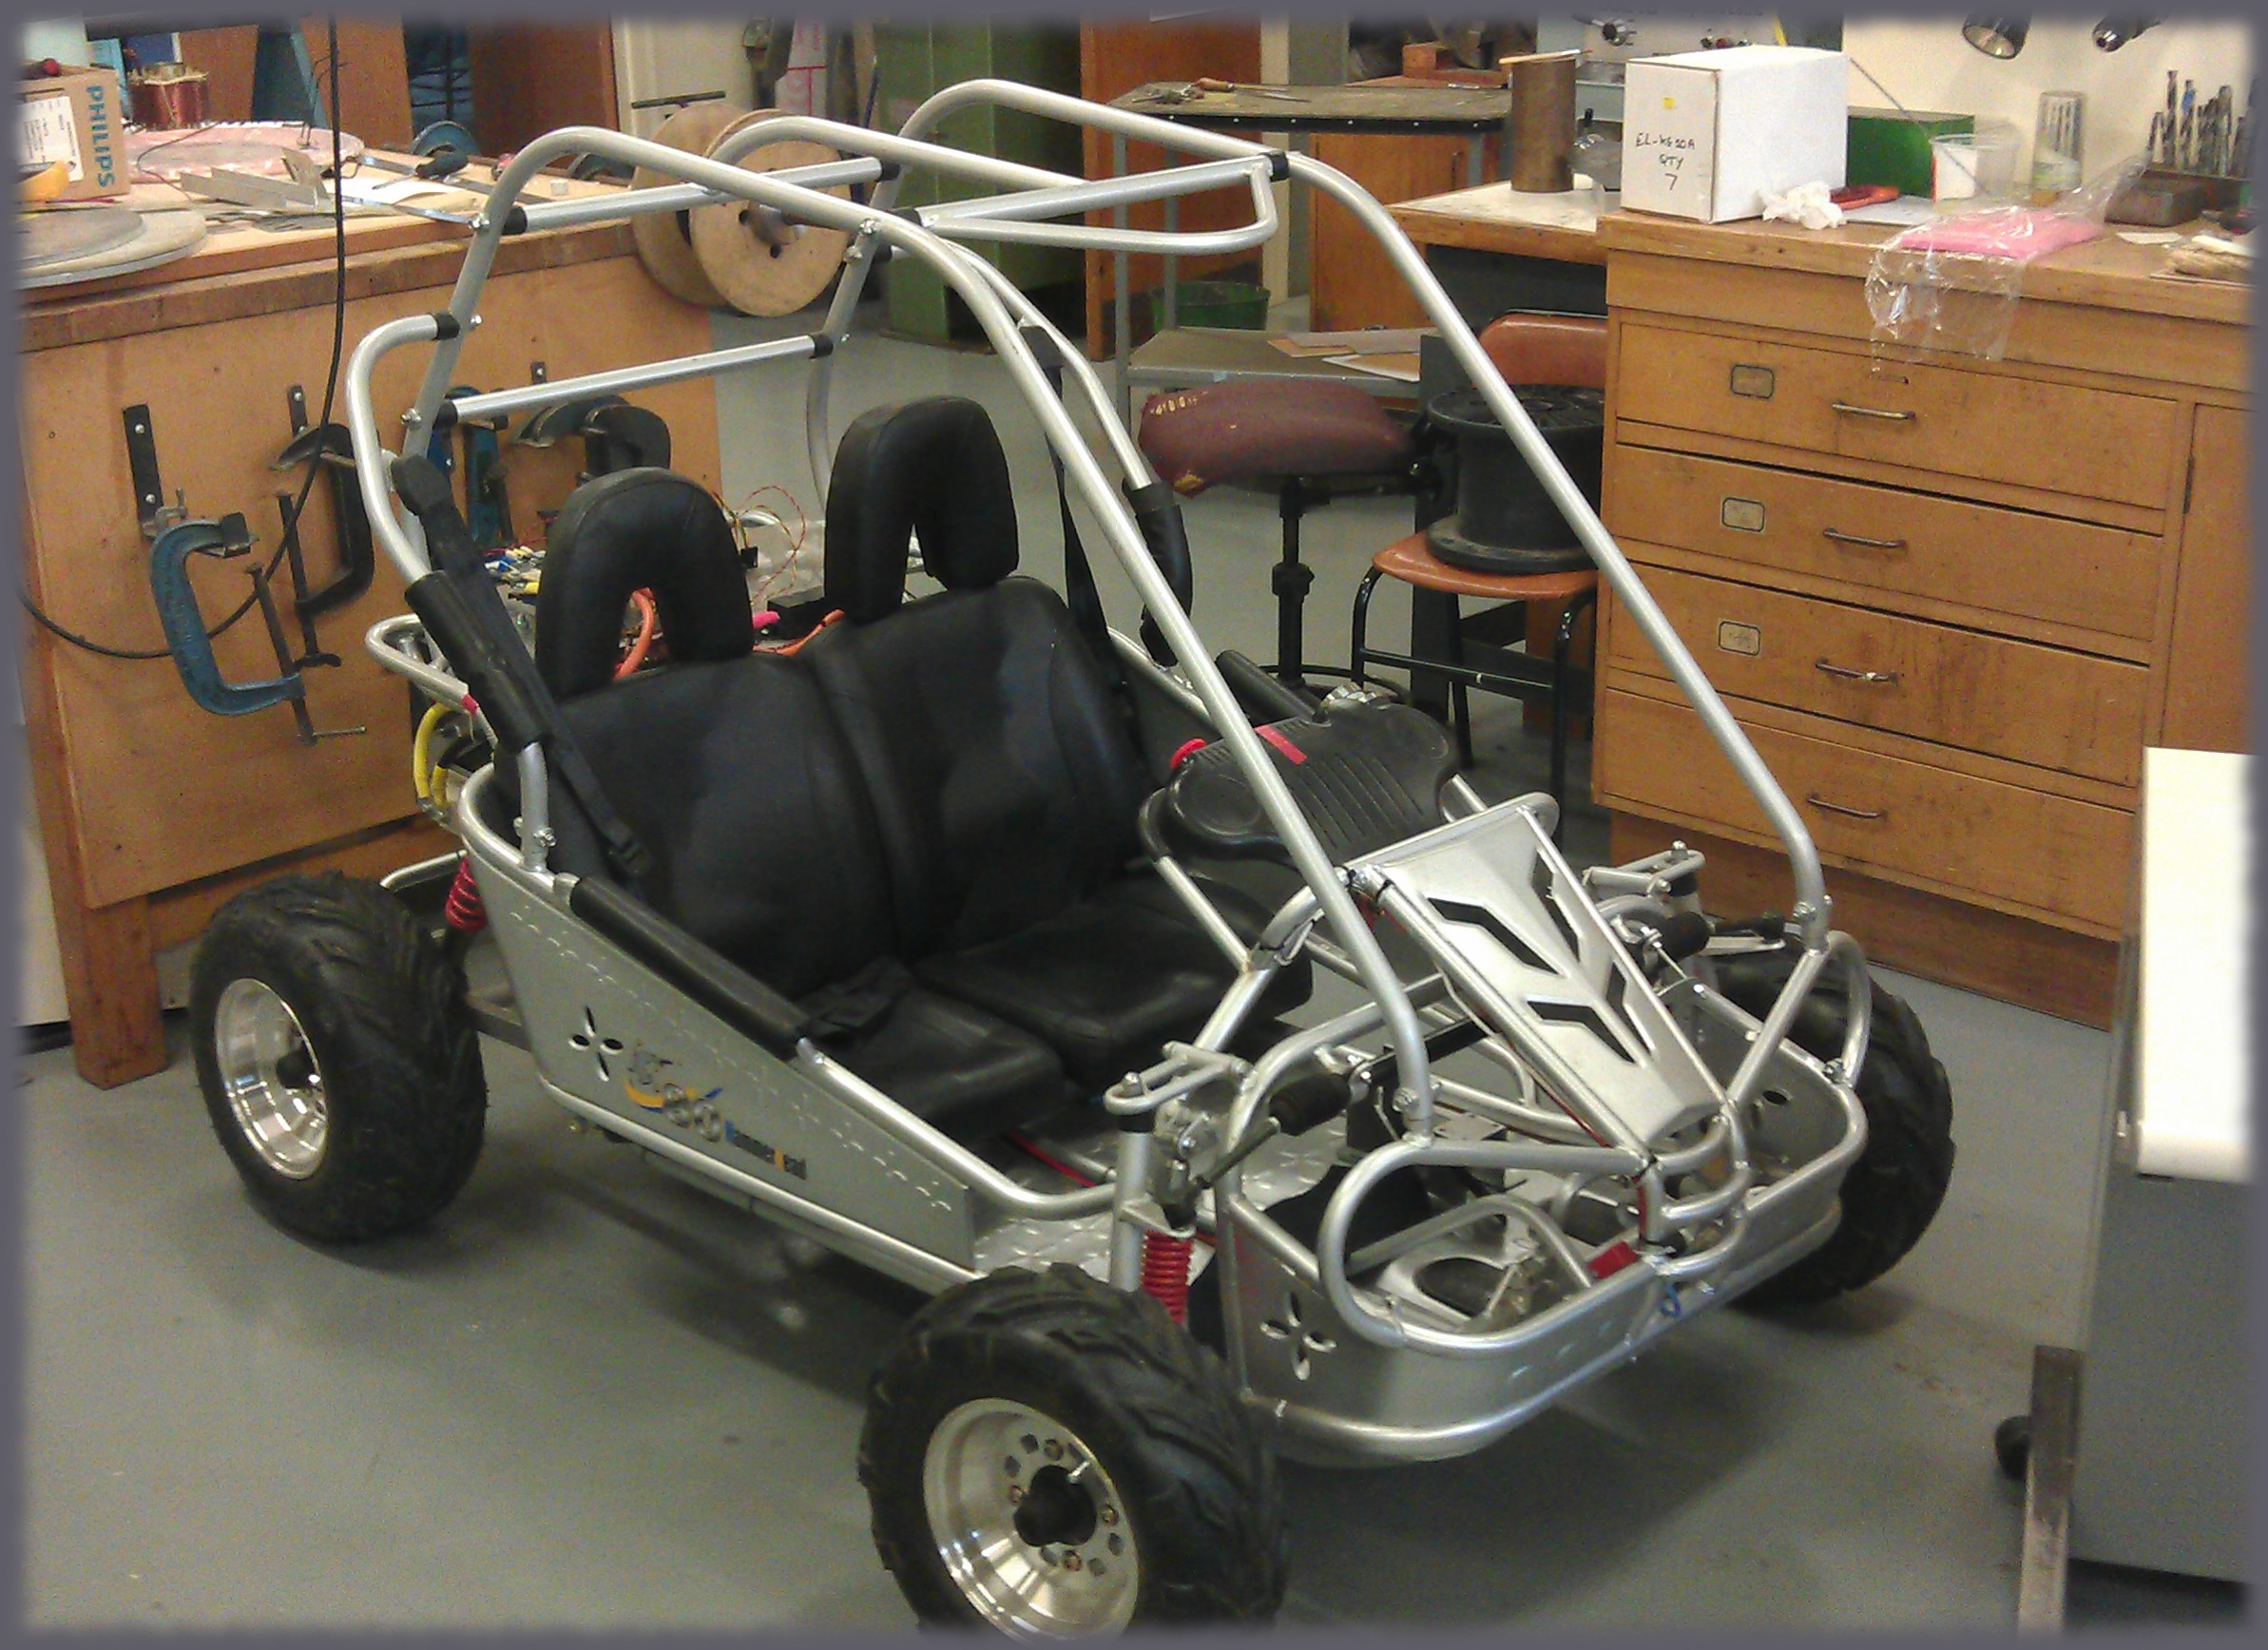
\includegraphics[width=.9\linewidth]{Images/kart.png}
      \caption[Junoir Sport - JS80IIR go-kart]{Electrical and Computer
      Engineering go-kart}
      \label{go-kart}
  \end{figure}


\subsection{Power Supply}
  The go-kart has a single power source for the whole vehicle. Two lead-acid
  batteries provide power for the existing DC drive motor and power electronics.
  These batteries can handle large currents at a voltage ranging up to 26 volts.
  The batteries have also been made accessible to be used for the autonomous
  vehicle control system.

\subsection{Power Electronics}
  To control the DC Drive motor, the department has come up with three PCBs to
  switch and regulate currents going through the motor. Figure \ref{powerE}
  shows the three PCBs, where from left to right they are the \emph{student
  board}, \emph{control saftey board} and \emph{power electronics board}. The
  student board is a 5V logic board that takes the possition of the accelerator
  pedal, current sensor data and outputs a PWM signal for the control safety
  board. The control safety board is there to make sure the power electronics
  board is not incorrectly driven, which would damage the go-kart.

  \begin{figure}[h]
      \centering
      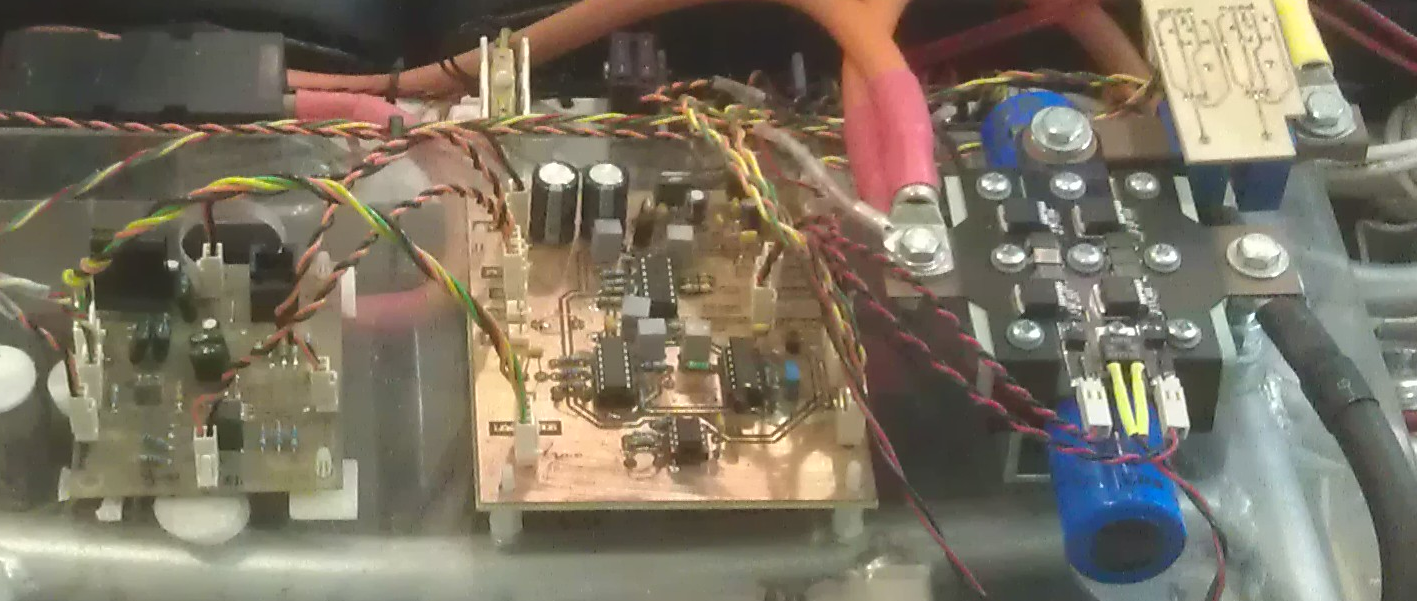
\includegraphics[width=.9\linewidth]{Images/powerE.png}
      \caption{Power and control electronics for go-karts DC motor}
      \label{powerE}
  \end{figure}

\subsection{Actuator Control}
  To control the steering position and apply the brakes two actuators were
  purchased for the project.

  \subsubsection{Steering}
    The steering motor is a 24V DC motor that has a step down gear box with an
    output ratio of 393:1. On the top end of the motor, there is an magnetic
    encoder that outputs 18 pulses per motor revolution. This is that it outputs
    7,074 pulses per 360 degrees of rotation on the steering wheel.

  \subsubsection{Brake}
    To control the possition of the brake a linear actuator was used. The linear
    actuator has an extension of 101.6mm and can travel at $20mm/s$. It provides
    absolout possition feedback via a $10k\ohm$ potentiometer.

\subsection{Communication With A Laptop}
  Because most laptops have dropped all serial RS-232 ports, the only
  reliable option for serial communications is to use USB. This also conforms as
  in the future USB web-cams can be used as sensors.

